\section{Naïvely Looking at the Poset Structure}
\label{tree:xy:grid}

In the \XY problem, we are asked to find a linear extension of a known partial
order having a specific structure. The \XY problem is thus a special case of
Sorting under Partial Information. In \ref{tree:supi}, we have seen that there
are algorithms solving the SUPI problem in \BigO{\log e(P)} comparisons. We
wonder if it is possible to prove that, if we are only allowed to exploit the
grid structure of a \XY poset, then \XY cannot be solved in less than \BigO{n^2
\log n} comparisons.

We already saw that the Hasse diagram of the poset \XY can be drawn as a grid.
This grid is finite and has a \(\hat{0}\) and a \(\hat{1}\). Moreover, every
two elements of this grid have a unique infimum and supremum. When this three
conditions are met for a poset, we call this poset a bounded lattice. We say
that the poset \XY is a \( n \times n \) bounded lattice.

We show that,

\begin{theorem}
The number of linear extension of the \( n \times n \) lattice is,
\begin{displaymath}
e(P) = \frac{(n^2)!}{\prod_{k=1}^{2n-1} k^{n - \abs{n-k}}}
\end{displaymath}
\end{theorem}

note that one can use the superfactorial notation
\( \sf(n) = n!\,(n-1)!\ldots 3!\,2!\,1! \)
to make the formula slimmer,

\begin{displaymath}
e(P) = \frac{(n^2)! \, \sf(n-1)^2}{\sf(2n-1)}
\end{displaymath}

To do so, we introduce the notion of Ferrers diagrams and standard Young tableaux.

A Ferrers diagram can be seen as a set of square tiles arranged in a square
box. They are arranged so that there cannot be any space between two tiles
lying on the same row or column and there can never be a row that contains more
tiles than another row above it. Moreover there cannot be space left between
the left side of the box and the first tile of each row. An example of a
Ferrers diagram is given in \ref{fig:xy:lattice:ferrers}.

A Young tableau is a special kind of numerotation of the tiles of a Ferrers
diagram. If a Ferrers diagram is made of $n$ tiles, then a Young tableau drawn
on this diagram will number its tiles from $1$ to $n$. We will add the
condition that if one reads tile numbers of rows (from left to right) or
columns (from top to bottom) one should only encounter increasing sequences of
numbers. We refer to Young tableaux respecting this condition as standard Young
tableaux. An example of a standard Young tableau is given in
\ref{fig:xy:lattice:young}.

\begin{figure}
\centering
\begin{subfigure}[b]{0.49\textwidth}
\centering
	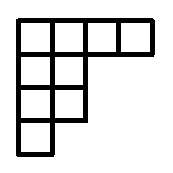
\includegraphics[width=0.4\textwidth]{fig/x+y/lattice/ferrers}
	\caption{Example of a Ferrers diagram with $9$ tiles. The shape of this
diagram is \(\lambda = (4,2,2,1)\).}
	\label{fig:xy:lattice:ferrers}
\end{subfigure}
\begin{subfigure}[b]{0.49\textwidth}
\centering
	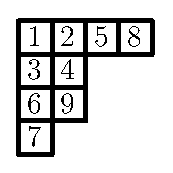
\includegraphics[width=0.4\textwidth]{fig/x+y/lattice/young}
	\caption{Example of a standard Young tableau in the Ferrers diagram of
\ref{fig:xy:lattice:ferrers}.}
	\label{fig:xy:lattice:young}
\end{subfigure}
\end{figure}

The number of standard Young tableaux for a given Ferrers diagram shape
\(\lambda\) can be computed using the hook-length formula \(d_{\lambda}\),

\begin{theorem}
\label{theorem:xy:lattice:hook}
Let \(\lambda = (\lambda_1,\ldots,\lambda_m)\) be a partition of the natural
number \(n\), \ie such that \(\sum_i \lambda_i = n\). The number of standard
Young tableaux of shape \(\lambda\) is
\begin{displaymath}
d_{\lambda} = \frac{n!}{\prod_{(i,j) \in \lambda} h_{\lambda}(i,j)}
\end{displaymath}
\end{theorem}

\(h_{\lambda}(i,j)\) denotes the length of an imaginary \emph{hook} bending at
\((i,j)\). The hook \(H_{\lambda}(i,j)\) is a subset of the tiles of
\(\lambda\) containing all tiles \((a,b)\) such that \(a = i\) and \(b \ge j\)
or \(b = j\) and \(a \ge i\). \ref{fig:xy:lattice:hooks} shows the hook length
at each tile and highlights the hook bending at \((2,1)\).

\begin{figure}
\centering
\begin{subfigure}[b]{0.49\textwidth}
\centering
	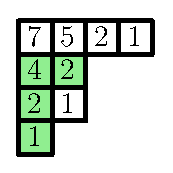
\includegraphics[width=0.4\textwidth]{fig/x+y/lattice/hooks}
	\caption{Ferrers diagram with hook length for each tile. The highlighted
region is the hook bending at \((2,1)\)}
	\label{fig:xy:lattice:hooks}
\end{subfigure}
\begin{subfigure}[b]{0.49\textwidth}
\centering
	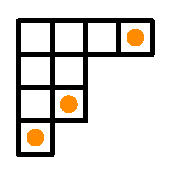
\includegraphics[width=0.4\textwidth]{fig/x+y/lattice/corners}
	\caption{Ferrers diagram with corners highlighted.}
	\label{fig:xy:lattice:corners}
\end{subfigure}
\end{figure}

The hook-length formula is attributed to \citet*{frame:1954}.Multiple ways to
prove \ref{theorem:xy:lattice:hook} are available in the literature. For more
information, one could start with \citet*{greene:1979} which gives a very nice
probabilistic proof and pointers for further reading.

We give a little insight into the proof found in \citet*{greene:1979}.
\ref{fig:xy:lattice:corners} highlights corners of a Ferrers diagram. A Young
tableau drawn in this diagram can only have its maximal element arranged in
one of these corner tiles, otherwise we would obtain a row or a column that is
not increasing. The number of ways of arranging the Young tableau in the
Ferrers diagram of shape \(\lambda\) is thus the sum of possible tableaux of
size \(n-1\) over all shapes \(\lambda \setminus \gamma\) where the maximal
element of our tableau of size \(n\) was put in corner \(\gamma\) of
\(\lambda\). Hence, the recurrence
\begin{equation}\label{equation:xy:lattice:reccurence}
d_{\lambda} = \sum_{\gamma \text{ is a corner of } \lambda} d_{\lambda
\setminus \gamma}
\end{equation}
holds. We can rewrite \ref{equation:xy:lattice:reccurence} as

\begin{equation}\label{equation:xy:lattice:walk}
\sum_{\gamma \text{ is a corner of } \lambda} \frac{d_{\lambda
\setminus \gamma}}{d_{\lambda}} = 1
\end{equation}

\citet*{greene:1979} define a hook walk to be a random walk starting at
any tile in the Ferrers diagram such that at each step, one moves uniformly at
random to an other tile of the hook bending at the current tile.
They show that each term of the sum in \ref{equation:xy:lattice:walk} is just
the probability for a single hook walk to end in each of the corners, proving
the theorem.

A \( n \times n \) bounded lattice can be regarded as a \( n \times n \)
standard Young tableau, i.e. a Young tableau of shape
\( \lambda = \enum{ \lambda_1 , \ldots , \lambda_n } \)
with
\( \lambda_i = n, \Forall i = 1 \ldots n \)
. Hence, we have
\( d_{\lambda} = e(P) \). \ref{fig:xy:lattice:xyhooks} shows the hook lengths
for the \( n \times n \) lattice, and thus for the \XY poset.

\begin{figure}
\centering
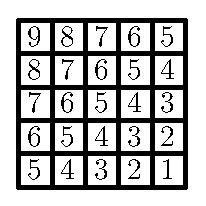
\includegraphics[width=0.3\textwidth]{fig/x+y/lattice/xyhooks}
\caption{Hook lengths for the \( n \times n \) lattice.}
\label{fig:xy:lattice:xyhooks}
\end{figure}

We still need to show that counting tableaux is the same as counting linear
extensions. We etiquette all \( n^2 \) nodes of \(P\), the Hasse Diagram of
\XY, with the numbers \(1\) to \( n^2 \) in any order. Suppose that we are
given a unique linear extension of \(P\) that can be represented as a tuple
\( \omega = ( j_1 , \ldots , j_{n^2}) \)
with all \( j_i \) distinct and between \(1\) and \( n^2 \) using our
etiquettes. If we are given \( n^2 \) distinct elements \( x_1 \) to
\( x_{n^2} \) then according to our proof, there are \( d_{\lambda} \) ways to
fill our tableau with those elements and to each filled tableau corresponds a
unique linear extension designated by \(\omega\).

\nb{As a side note, the hook-length formula is closely related to
multidimensional Catalan numbers. The hook-length formula generates the numbers
on the diagonal of the matrix containing the \(\nth{n}\) \(m\)-dimensional
Catalan number at position \((m,n)\) \cite{OEIS:A060854}. The \(\nth{n}\)
\(m\)-dimensional Catalan numbers gives the number of shortest paths in the
\(m\)-dimensional unit grid from \( (0,\ldots,0) \) to \( (n,\ldots,n) \) such
that if \( (x_1,\ldots,x_m) \) is on a path then \( x_1 \le x_2 \le \ldots \le
x_m\).}

We now show that,

\begin{theorem}
\( \log e(P) = \BigO{n^2 \log n} \)
\end{theorem}

\begin{proof}
Using Stirling's approximation,
\begin{align}
e(P) &= \frac{(n^2)!}{1 \cdot 2 \cdot 2 \cdot \cdots \cdot (2n-2) \cdot (2n-2) \cdot (2n-1)}\\
e(P) &\ge \frac{(n^2)!}{(2n)^{n^2}}\\
\ln e(P) &\ge \ln \group{\frac{(n^2)!}{(2n)^{n^2}}}\\
\lim_{n \to \infty} \ln e(P) &\ge \ln{\group{\sqrt{2 \pi n^2}
\group{\frac{n^2}{\euler}}^{n^2}}}  - n^2 \ln n - n^2 \ln 2\\
\lim_{n \to \infty} \ln e(P) &\ge \ln{\sqrt{2\pi}} + \ln n - n^2 \ln e + 2 n^2
\ln n - n^2 \ln n - n^2 \ln 2\\
\lim_{n \to \infty} \ln e(P) &\ge n^2 \ln n - n^2 \ln (2\euler) + \ln n + \ln \sqrt{2\pi}
\end{align}
\end{proof}

Thus, solving \XY in \SmallO{n^2 \log n} comparisons is not possible if we only
consider the information contained in the poset structure, \ie if we only
exploit the fact that \( X_i \le X_{i'} \land Y_j \le \Y_{j'} \implies X_i +
Y_j \le X_{i'} + Y_{j'}\). Moreover, to sort a poset having the same structure,
the trivial mergesort technique explained earlier is optimal.
\ref{tree:xy:counting} shows that there is indeed more information available.
